





%%%%%%%%%%%%%%%%%%%%%%%%%%%%%%%%%%%%%%%%%%%%%%%%%%%%%%%%%%%%%%%%%%%%%%%%%%%
%%
%%  LaTeX + CJK 模板,只针对 A4 纸的中文Paper。
%%
%%  Ver 1.02 By DeathKing @ <dk.hit.edu.cn>
%%  Ver 1.01 By rabbitbug @ www.ctex.org
%%  Ver 1.0 by oLo @ bbs.ustc.edu.cn
%%
%%  You can mofify it and distribute it freely:)
%%
%%%%%%%%%%%%%%%%%%%%%%%%%%%%%%%%%%%%%%%%%%%%%%%%%%%%%%%%%%%%%%%%%%%%%%%%%%%%

%%%%%%%%%%%%%%%%%%%%%%%%%%%%%%%%%%%%%%%%%%%%%%%%%%%%%%%%%%%%%%%%
%  文章模板:A4 纸,小五字,单列(可根据要求改双列 twocolumn)
%%%%%%%%%%%%%%%%%%%%%%%%%%%%%%%%%%%%%%%%%%%%%%%%%%%%%%%%%%%%%%%%
\documentclass[a4paper,11pt,onecolumn,twoside]{article}
\usepackage{CJK}         
\usepackage{fancyhdr}
\usepackage{amsmath,amsfonts,amssymb,graphicx}    
\usepackage{subfigure}   
\usepackage{indentfirst} 
\usepackage{bm}          
\usepackage{multicol}    
\usepackage{indentfirst} 
\usepackage{picins}      
\usepackage{abstract}    
\addtolength{\topmargin}{-54pt}
\setlength{\oddsidemargin}{-0.9cm}  
\setlength{\evensidemargin}{\oddsidemargin}
\setlength{\textwidth}{17.00cm}
\setlength{\textheight}{24.00cm}    
\renewcommand{\baselinestretch}{1.1}
\parindent 22pt 

\begin{CJK}{UTF8}{gbsn}
\title{\huge{Matlab 钢琴作曲}}
\author{吴田波~~荆潇\\[2pt]
\normalsize
(清华大学自动化系,自53班~学号~2015011428 ~~清华大学自动化系~~自53班~学号~2015011431) \\[2pt]}
\date{}  
\end{CJK}


\fancypagestyle{plain}{
\fancyhf{}
\lfoot{}
\cfoot{}
\rfoot{}}


\pagestyle{fancy}
\fancyhf{}
\fancyhead[LE,RO]{\thepage}
\lfoot{}
\cfoot{}
\rfoot{}

\newenvironment{figurehere}
  {\def\@captype{figure}}
  {}
\makeatother

\usepackage{titlesec}
\newcommand{\sectionname}{节}
\renewcommand{\figurename}{图}
\renewcommand{\tablename}{表}
\renewcommand{\contentsname}{目~录}
\renewcommand{\listfigurename}{图~目~录}
\renewcommand{\listtablename}{表~目~录}
\renewcommand{\indexname}{索~引}
\renewcommand{\abstractname}{\Large{摘~要}}
\newcommand{\keywords}[1]{\\ \\ \textbf{关~键~词}:#1}
\titleformat{\section}[block]{\large\bf}{\thesection}{10pt}{}
\begin{document}

\begin{CJK*}{UTF8}{gbsn}
\newcommand{\supercite}[1]{\textsuperscript{\cite{#1}}}
\maketitle

\setlength{\oddsidemargin}{ 1cm}  % 3.17cm - 1 inch
\setlength{\evensidemargin}{\oddsidemargin}
\setlength{\textwidth}{13.50cm}
\vspace{-.8cm}
\begin{center}
\parbox{\textwidth}{
\CJKfamily{hei}摘~~~要\quad \CJKfamily{kai}~本文将利用Matlab生成钢琴曲,本文将先对于网上已有的钢琴音频进行分析,记录了
基频频率以及前四个谐频的幅值。然后通过合成方式合成对应的曲调。最后通过这些曲调,加上本文具有创新的包络线降噪方式实现一个完整的曲子。\\
\CJKfamily{hei}关键词\quad\CJKfamily{kai}Matlab,FFT,包络线降噪\\}
\end{center}

\setlength{\oddsidemargin}{-.5cm}  % 3.17cm - 1 inch
\setlength{\evensidemargin}{\oddsidemargin}
\setlength{\textwidth}{17.00cm}
\CJKfamily{song}
\begin{multicols}{2}
\section{引言}
\indent Matlab是一个强大的数学软件。在对于信号的处理上Matlab也有极为出色的表现。音乐作为一个十分有意义的声音信号也是
经常被用于在信号分析上。本文将会介绍利用Matlab分析已有的钢琴标准音阶的频谱特性,并通过这个特性反向还原出钢琴的音符,并利用这音符进行作曲。\\
\indent 我们在本文将首先介绍有关钢琴音阶的基本原理,介绍有关十二平均律的基本知识。之后本文将介绍利用Matlab处理声音信号的基本方式,以及在
本文中采用的用于处理钢琴音的方法。之后再第二部分我们会介绍如何利用从处理钢琴音得到的频域信息中还原出钢琴音并能最终组成一部曲子,以及我们创新的使用了一个综合性的包络线。\\
\section{原理}


\subsection{有关钢琴和音乐的基本知识}

\normalsize
\indent 十二平均律是现代音乐理论体系的一个基本理论基础。其基本原理来说就是每相隔十二个音阶的音的基准频率相差2倍,并且每一个音阶相差的频率在对数坐标上是相等的,即每一级相差$2^{\frac{1}{12}}$倍的频率。这十二个音阶内的音在钢琴中被称为一个八度。
可以用字母表示为A,B,C,D,E,F,G,对应于简谱的1-7。但是如果要区分不同乐器的音色,还要考虑到谐音,即基频的倍数频的频率上幅值上的特征情况。因此如果要考虑较好的完整记录下钢琴音的信息可以
通过从网上开源音乐网站上找到的一个八度内的标准钢琴音,用Matlab进行分析记录特征。然后对于升调和降调则是通过直接基频增倍或是基频减半的方式实现。这样就可以获得基本上全部的音调。

\subsection {Matlab处理声音信号}
\indent Matlab是一个强大的数学分析软件,同时对于声音文件也有非常好的支持接口。直接利用Matlab内带的读取函数即可读取对应的信号。
接下来对于读取进来的音频信号尽心处理时,选择利用fft方法进行处理从而得到对应的频谱信息。虽然从理论上认为幅值最大的频率应该是信号的
基频信息,但实际上由于谐波混叠以及噪音的影响,一般来讲是二倍频处的幅值最大。另一方面,fft对应的是离散时间傅里叶变化的快速算法,如果要
使的横轴直接反应真实的频率信号和幅度,还需要做对应的处理。[1]设原始信号采样频率为 $F_s$,fft的采样点为N。则横轴x与竖轴y应该进行如下的变化:
\begin{equation}
			x^{'}=x*\frac{F_s}{N}-F_s/2
			y^{'}=y/(N/2)
\end{equation}
变化后的图像大致如下

\begin{figurehere}
\centering
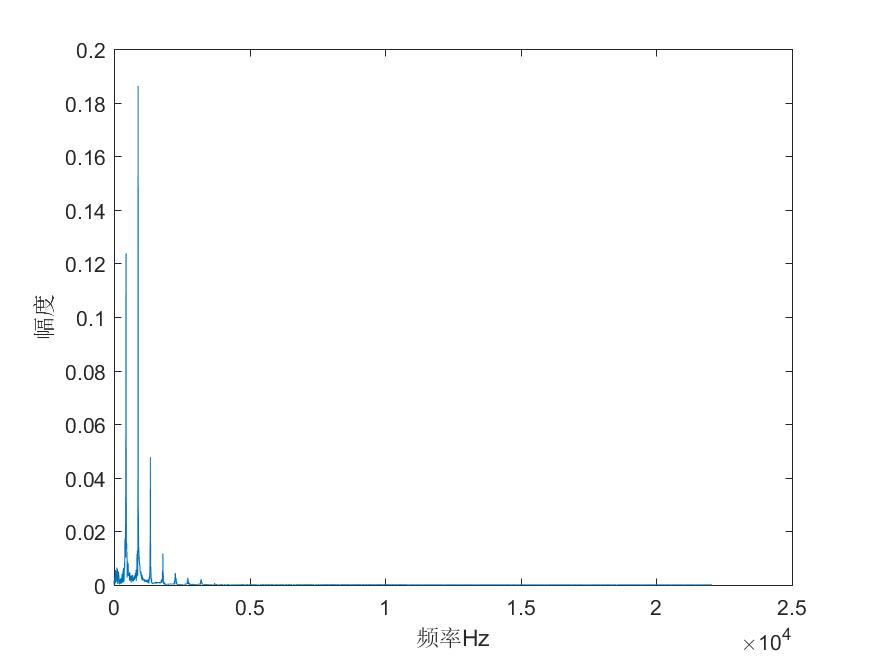
\includegraphics[width=6cm]{../source/source_jpg/piano_a.jpg} \caption{变化后的fft频谱图}\label{theory—s}
\end{figurehere}
通过这种方式可以较好的实现频域信息的读取。\\
\indent另一个要解决的问题是要选择哪些信息予以保存以便通过Matlab的声音生成函数反向生成得到钢琴音。有信号系统课程上的知识以及音乐乐理的相关
知识,只需要记录一个基频频率以及其谐频幅值较大的一部分的幅值即可,其余的信息应该被视为噪音而被滤去。这也是因为音乐的音在理论上是由基频和谐频组成的,其余的信息是录音时环境背景噪音带来的影响。\\

\subsection{Matlab还原音符和作曲}
\indent 对于还原主要有以下几个工作\\
\subsubsection{单个音调的合成}
\indent 通过对单个按键发音的频域分析,可以得到单个音调的基波、谐波及对应的幅值比例,将相应数据储存为向量,并进行傅里叶级数合成,得到单个按键音调的模拟。考虑到真实按键发音中,含有低频噪音,从而相对圆润,故加入低频分量。\\
\subsubsection{包络线模拟音色}
单个音调在合成过程中,由于持续发音时间内,信号幅度没有衰减,从而显得单调而不真实。通过加入指数型衰减信号作为包络线,可以较好的模拟音色。
但是,在初步合成音乐的过程中,发现会有“啪”的噪音,这是由于音调之间切换时,会从0跳跃到某个值,从而产生噪音。通过分析真实的钢琴音调的频率衰减,近似采用折线型包络线。这也是本文主要创新之处[2]
最后综合产生的包络线形状如下所示
\begin{figurehere}
\centering
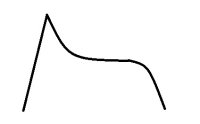
\includegraphics[width=6cm]{../source/theory.jpg}\caption{包络线示意图}\label{fold}
\end{figurehere}
实现该包络线的主要原理就是实现包络线矩阵T,而假设原有的傅里叶级数合成的声音信号矩阵为A;则最终的时域信号Y有:
$Y=A.*T$\\
\subsubsection{合成简单音乐}
通过十二平均律,根据分析得到的各个音调的基波、谐波频率和幅值,而通过简谱信息可以得到以及各个音调持续的节拍数,并根据一般音乐节奏
确定每个节拍的时间宽度一及两个节拍之间的时间间隔。从而能够进行音调的合成。简而言之:就是基于单个音调的合成,加上时间信息合成简单的乐曲
并且通过包络线方法进行降噪。\\
\subsubsection{音乐升降度处理}
由于简谱的音调虽然主要在一个八度内,但有时仍会有高八度或低八度的音出现,此时需要进行处理。根据十二平均律,对于高八度的音或低八度的音,通过基波频率乘2或除以2来实现。\\

\section{仿真测试结果}
\subsection{钢琴音的Matlab分析}
利用Matlab分析钢琴的中档的A-G的七个音符的频谱图片如下
\begin{figurehere}
\centering
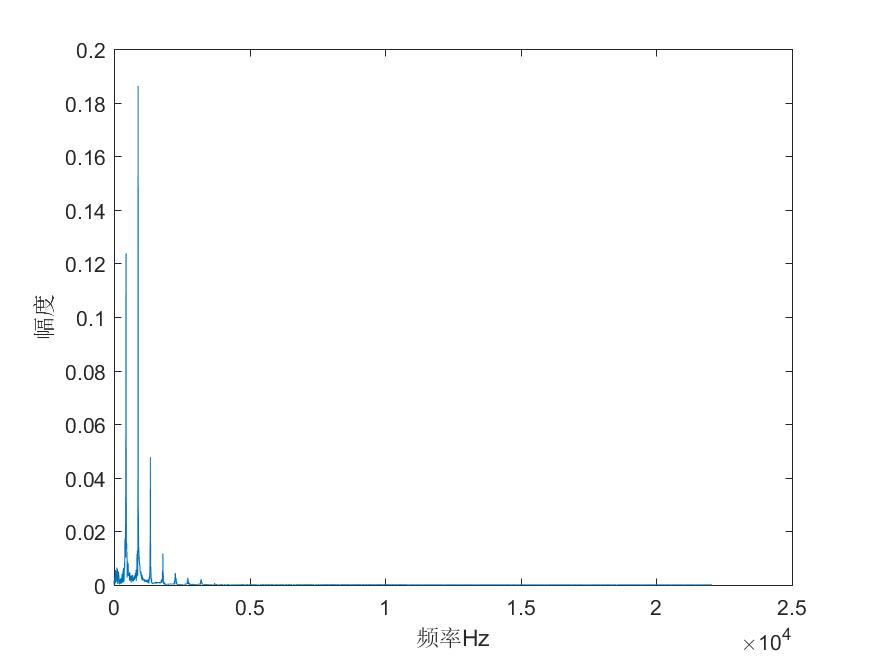
\includegraphics[width=6cm]{../source/source_jpg/piano_a.jpg}\caption{A的频域图}\label{A}
\end{figurehere}
\begin{figurehere}
\centering
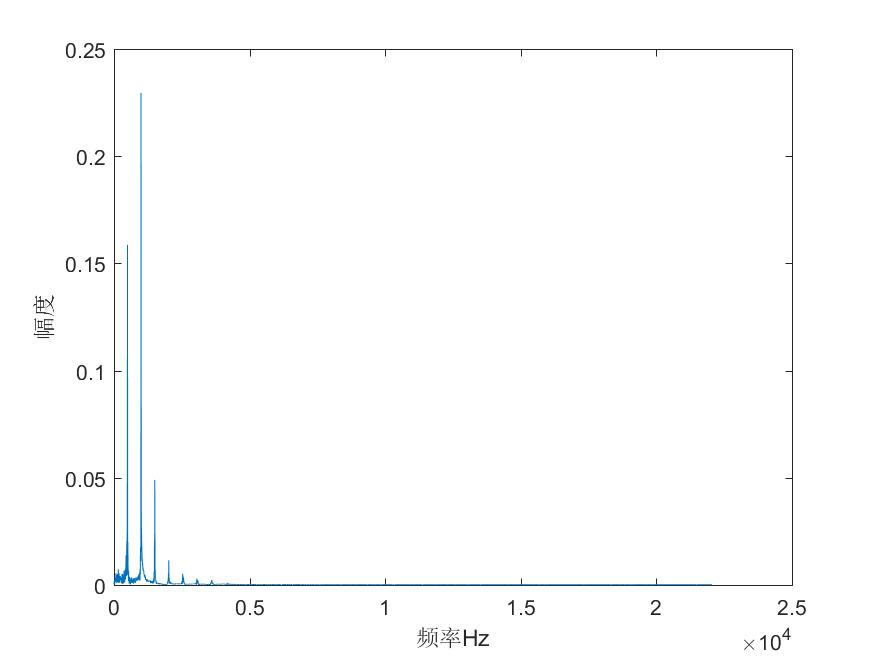
\includegraphics[width=6cm] {../source/source_jpg/piano_b.jpg}\caption{B的频域图}\label{B}
\end{figurehere}
\begin{figurehere}
\centering
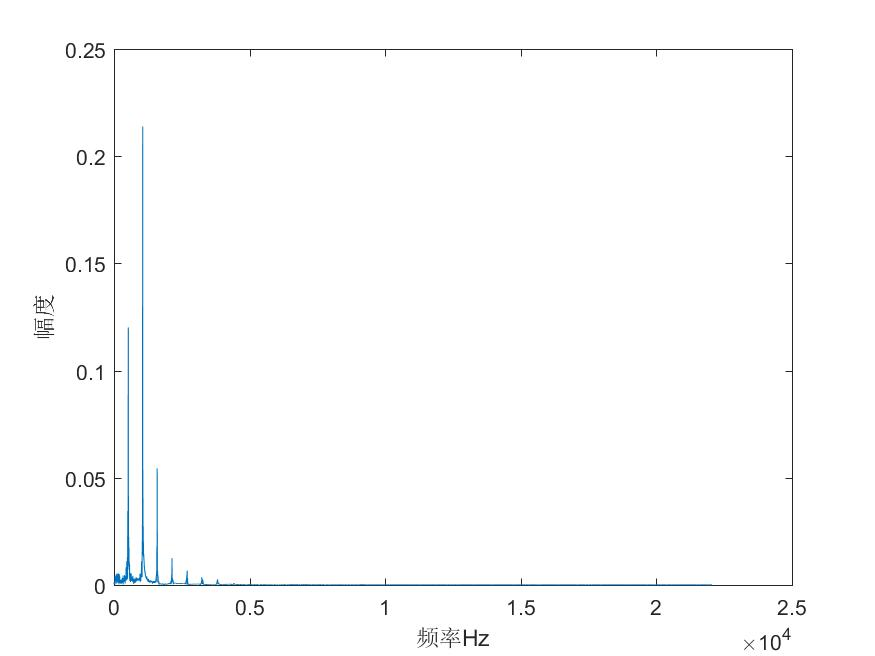
\includegraphics[width=6cm]{../source/source_jpg/piano_c.jpg}\caption{C的频域图}\label{C}
\end{figurehere}
\begin{figurehere}
\centering
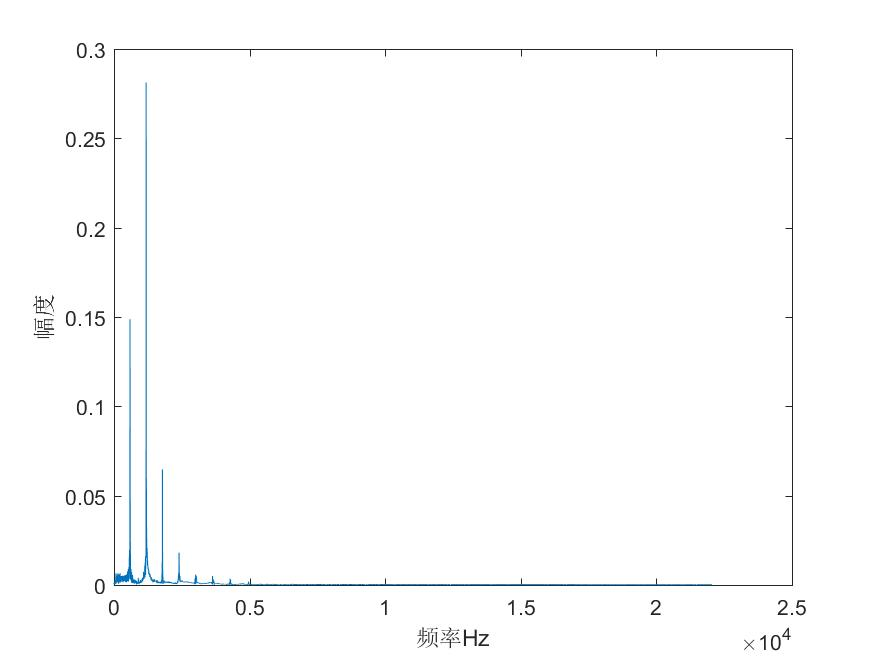
\includegraphics[width=6cm]{../source/source_jpg/piano_d.jpg}\caption{D的频域图}\label{D}
\end{figurehere}
\begin{figurehere}
\centering
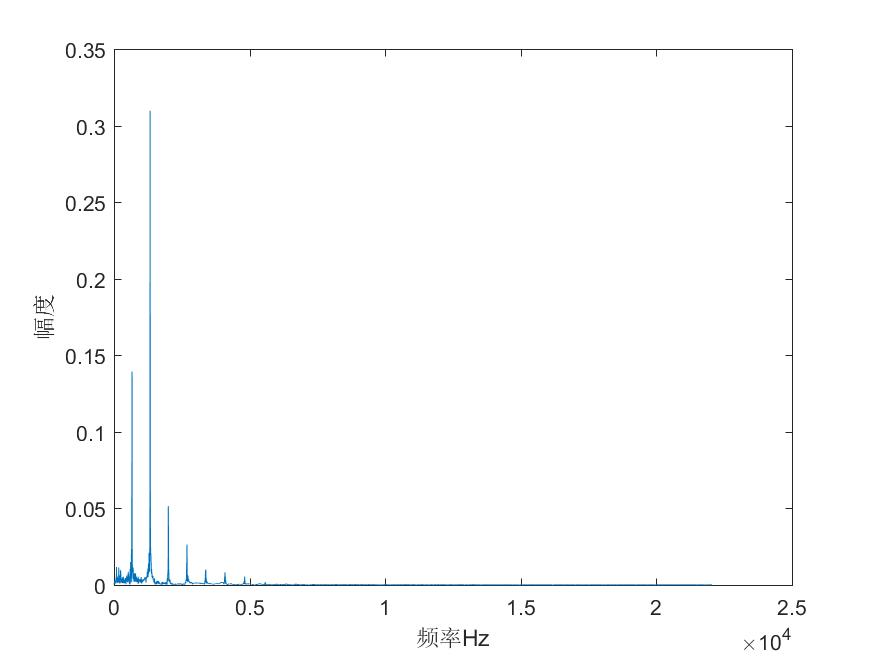
\includegraphics[width=6cm]{../source/source_jpg/piano_e.jpg}\caption{E的频域图}\label{E}
\end{figurehere}
\begin{figurehere}
\centering
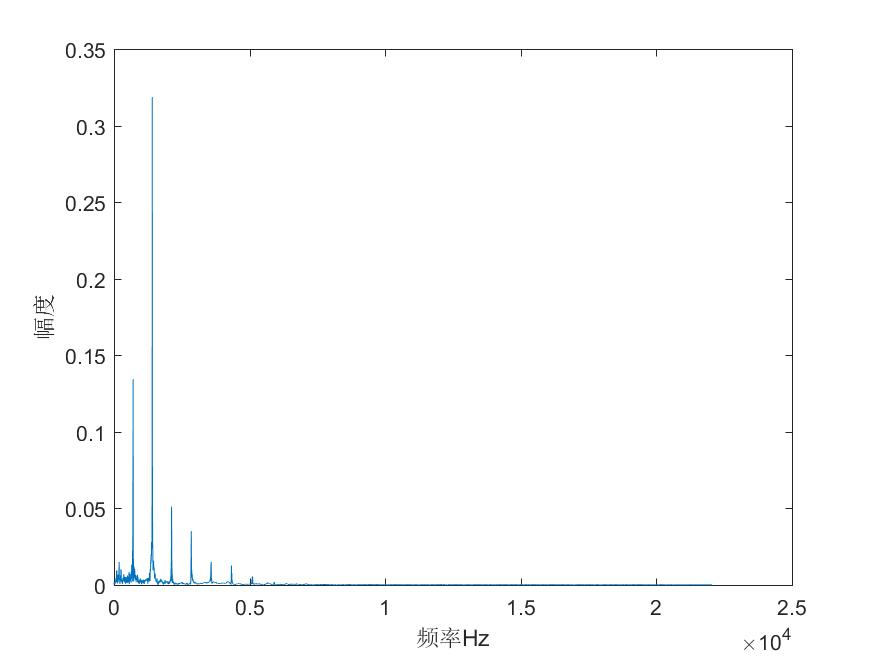
\includegraphics[width=6cm]{../source/source_jpg/piano_f.jpg} \caption{F的频域图}\label{F}
\end{figurehere}
\begin{figurehere}
\centering
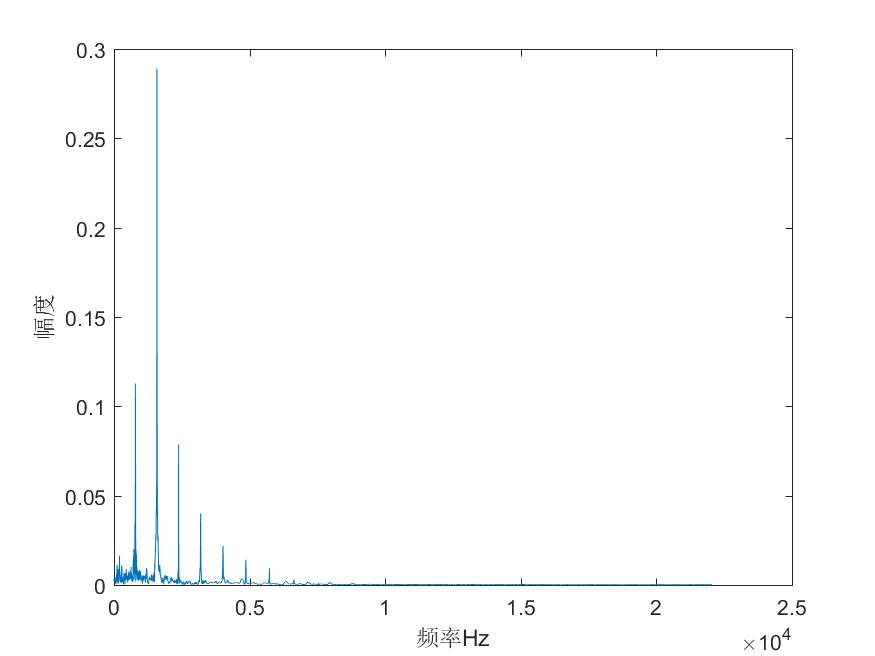
\includegraphics[width=6cm]{../source/source_jpg/piano_g.jpg} \caption{G的频域图}\label{G}
\end{figurehere}
然后整理记录的数据表格如下,主要记录各个音符的基频频率,以及前面三个谐波频率的幅值(小于0.01的幅值部分记录为零)
\begin{tabular}{ccc}
		\hline
		音符名& 基频频率 & 基频幅值 & 二倍频幅值 &三倍频幅值 &四倍频幅值\\
		\hline
		A &441 &0.1206 &0.1862 &0.04764 &0.01175\\
		\hline
		B	&498.3 & 0.1586 &0.2295 &0.04901  &0\\
		\hline
		C	&524.8 &0.1193 &0.2139 &0.05438  &0\\
		\hline
		D	&590.9 &0.1487 &0.2813 &0.0647   &0\\
		\hline
		E &665.9 &0.1393 &0.3097 &0.05142  &0\\
		\hline
		F &705.6 &0.1344 &0.3186 &0.5116   &0\\
		\hline
		G	&789.4 &0.1128 &0.2899 &0.07855  &0.03796\\
		\hilne
\end{tabular}
该结果与网上已有的结果相比较为接近,是一个可以接受的结果。
\subsection{Matlab合成简单的音乐}
\subsubsection{基本的音调}
将之前一步的结果存储在文本文件中,然后在本次操作中进行读取操作,之后用傅里叶级数的形式合成单独的音调。
单独音调的时域图如下所示:
\begin{figurehere}
\centering
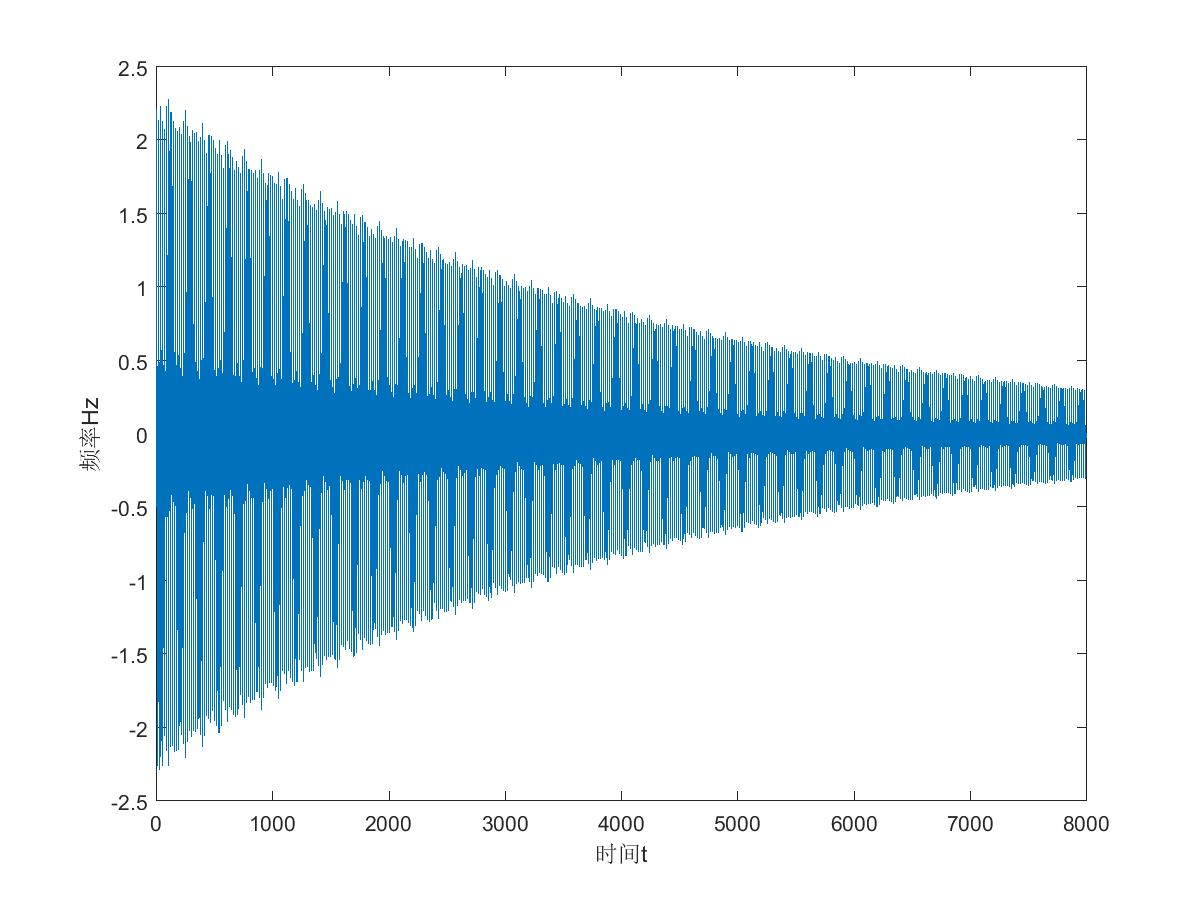
\includegraphics[width=6cm]{../source/generate_jpg/tone_a.jpg}\caption{生成的A时域域图} \label{at}
\end{figurehere}
\begin{figurehere}
\centering
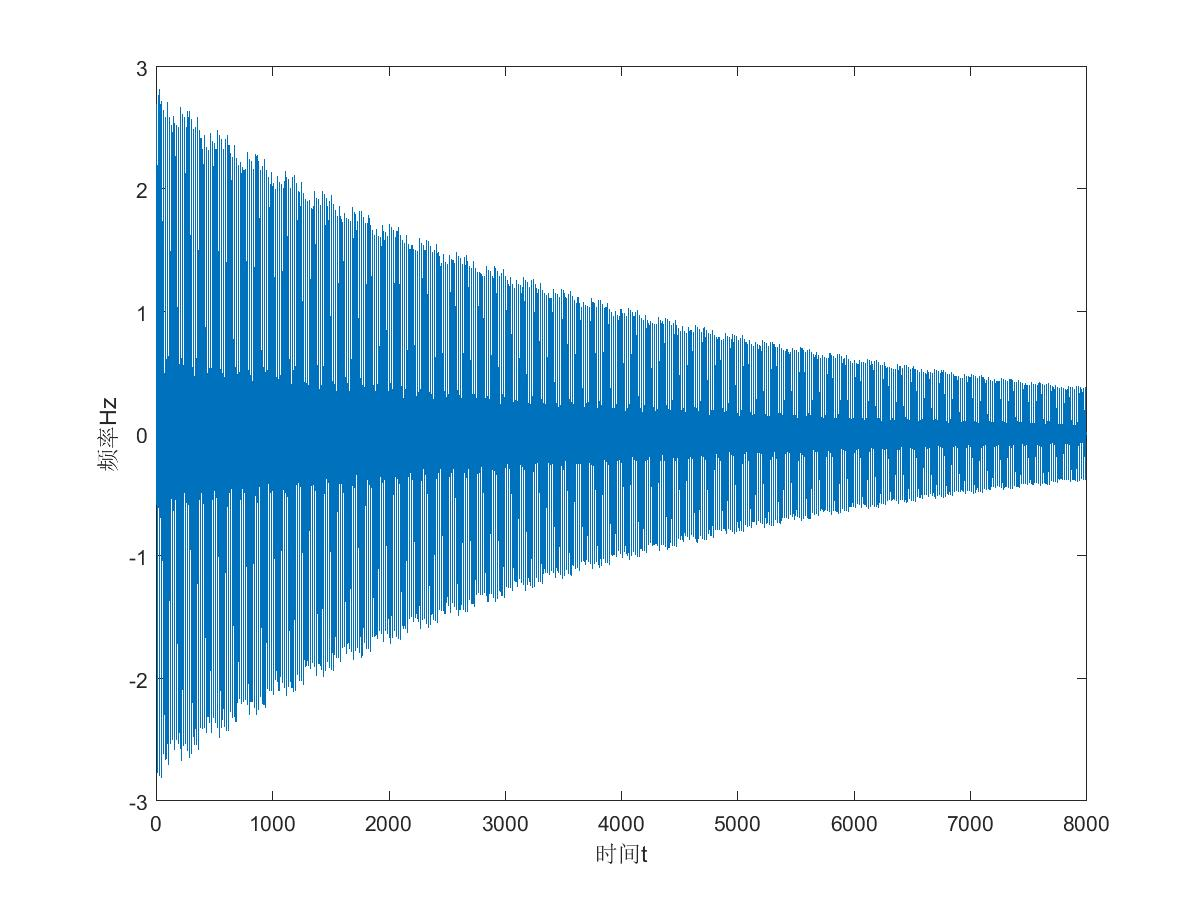
\includegraphics[width=6cm]{../source/generate_jpg/tone_b.jpg}\caption{生成的B时域域图} \label{bt}
\end{figurehere}
\begin{figurehere}
\centering
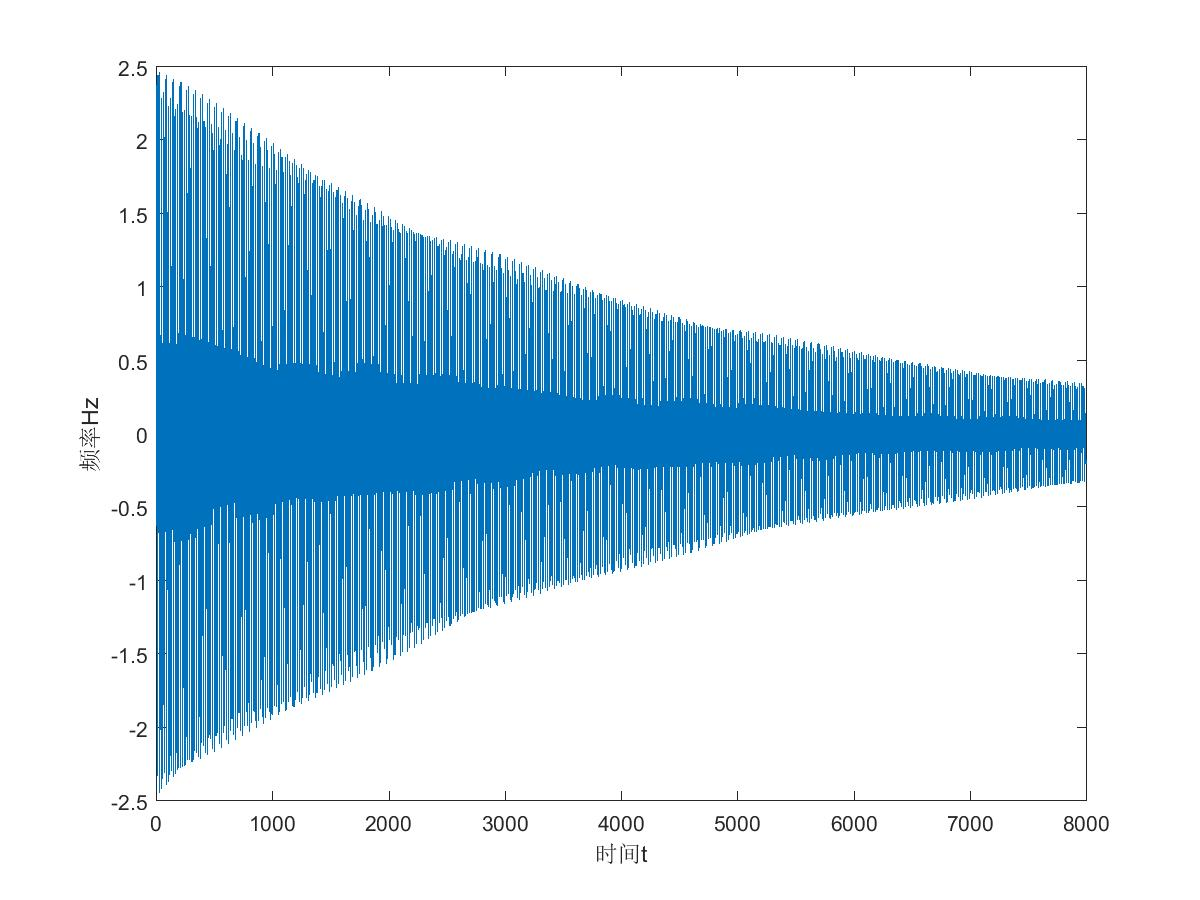
\includegraphics[width=6cm]{../source/generate_jpg/tone_c.jpg}\caption{生成的C时域域图}\label{ct}
\end{figurehere}
\begin{figurehere}
\centering
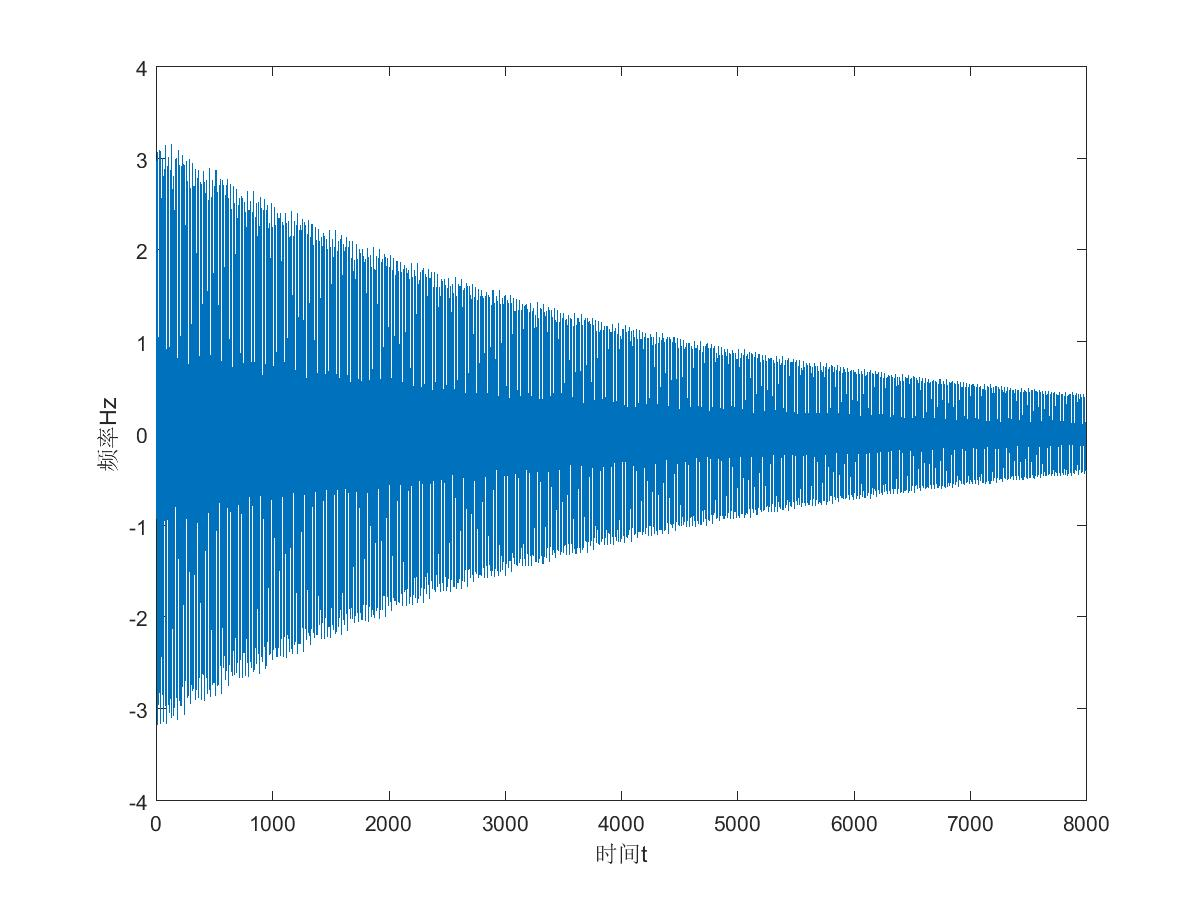
\includegraphics[width=6cm]{../source/generate_jpg/tone_d.jpg}\caption{生成的D时域域图}\label{dt}
\end{figurehere}
\begin{figurehere}
\centering
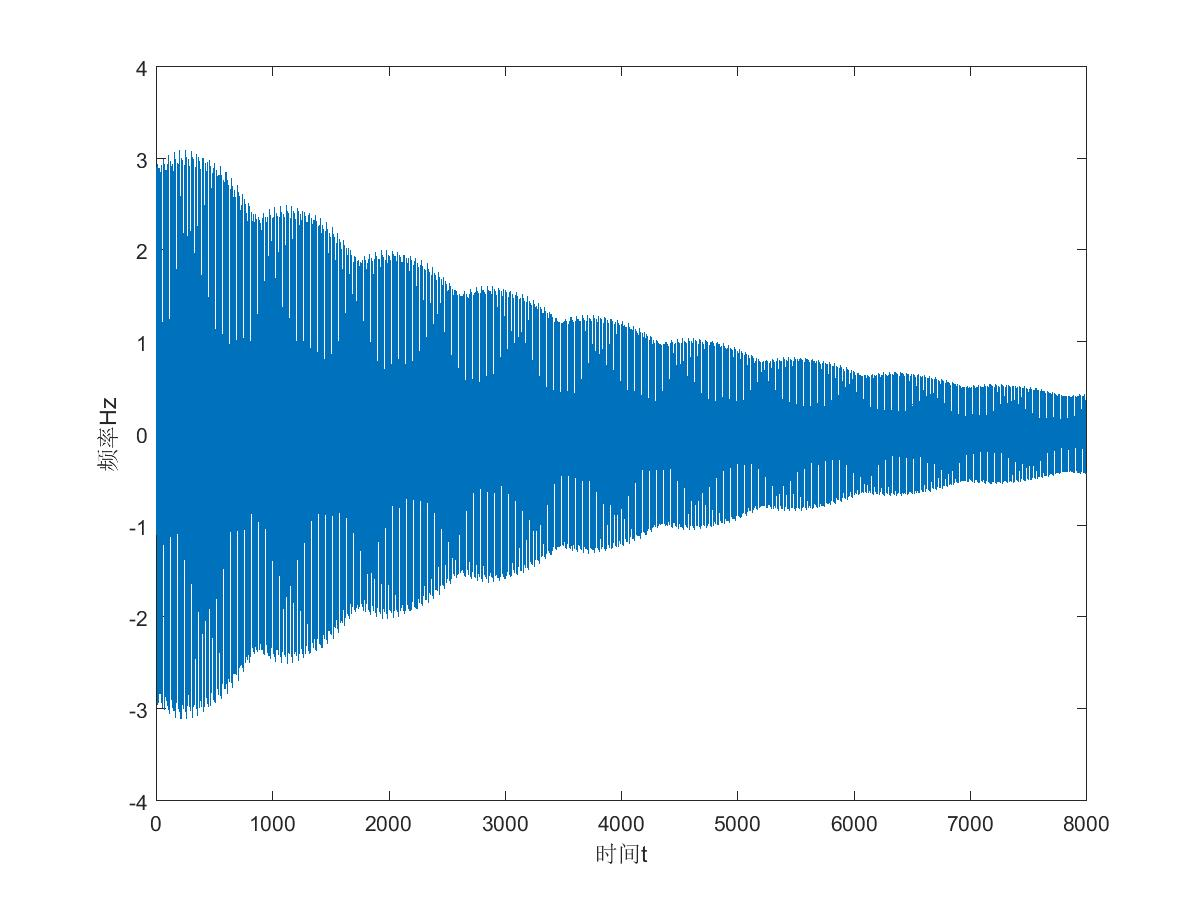
\includegraphics[width=6cm]{../source/generate_jpg/tone_e.jpg}\caption{生成的E时域域图}\label{et}
\end{figurehere}
\begin{figurehere}
\centering
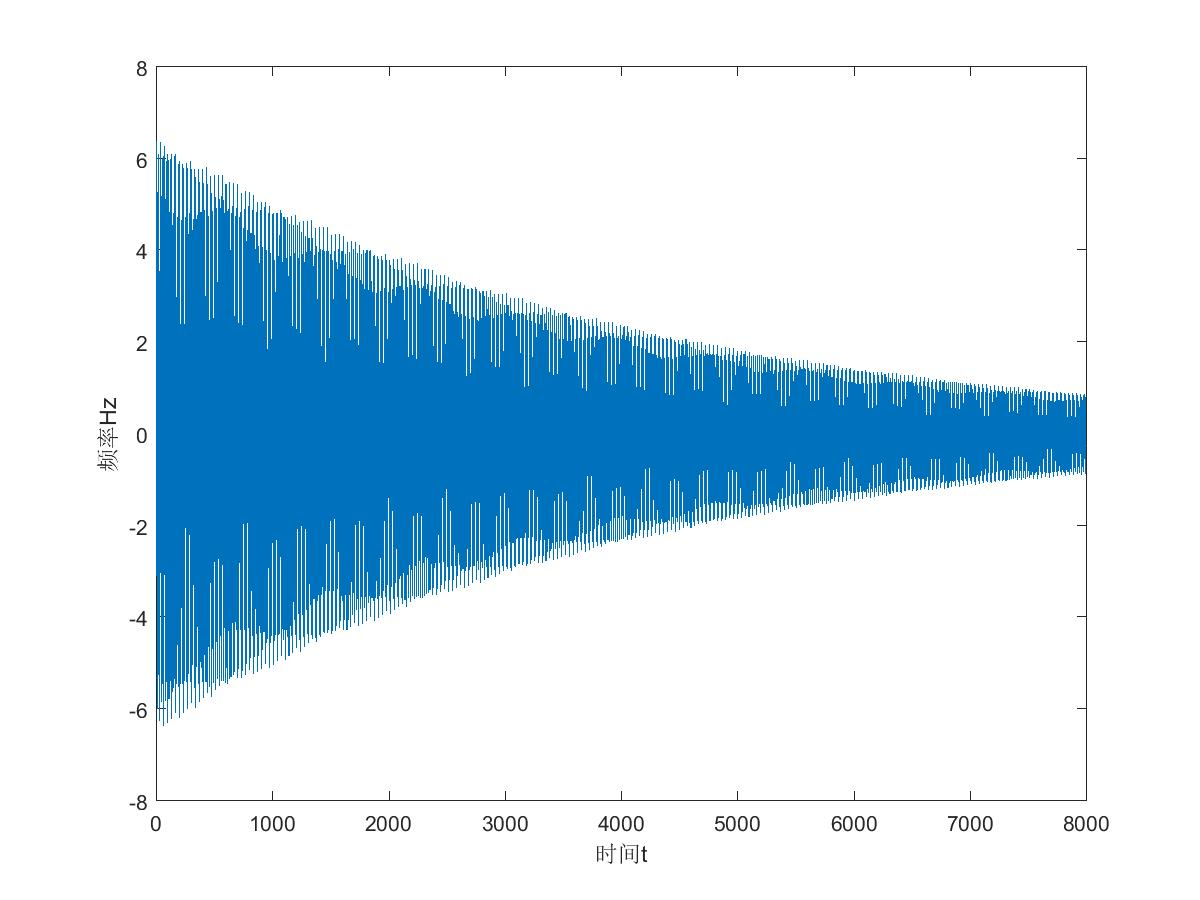
\includegraphics[width=6cm]{../source/generate_jpg/tone_f.jpg}\caption{生成的F时域域图}\label{ft}
\end{figurehere}
\begin{figurehere}
\centering
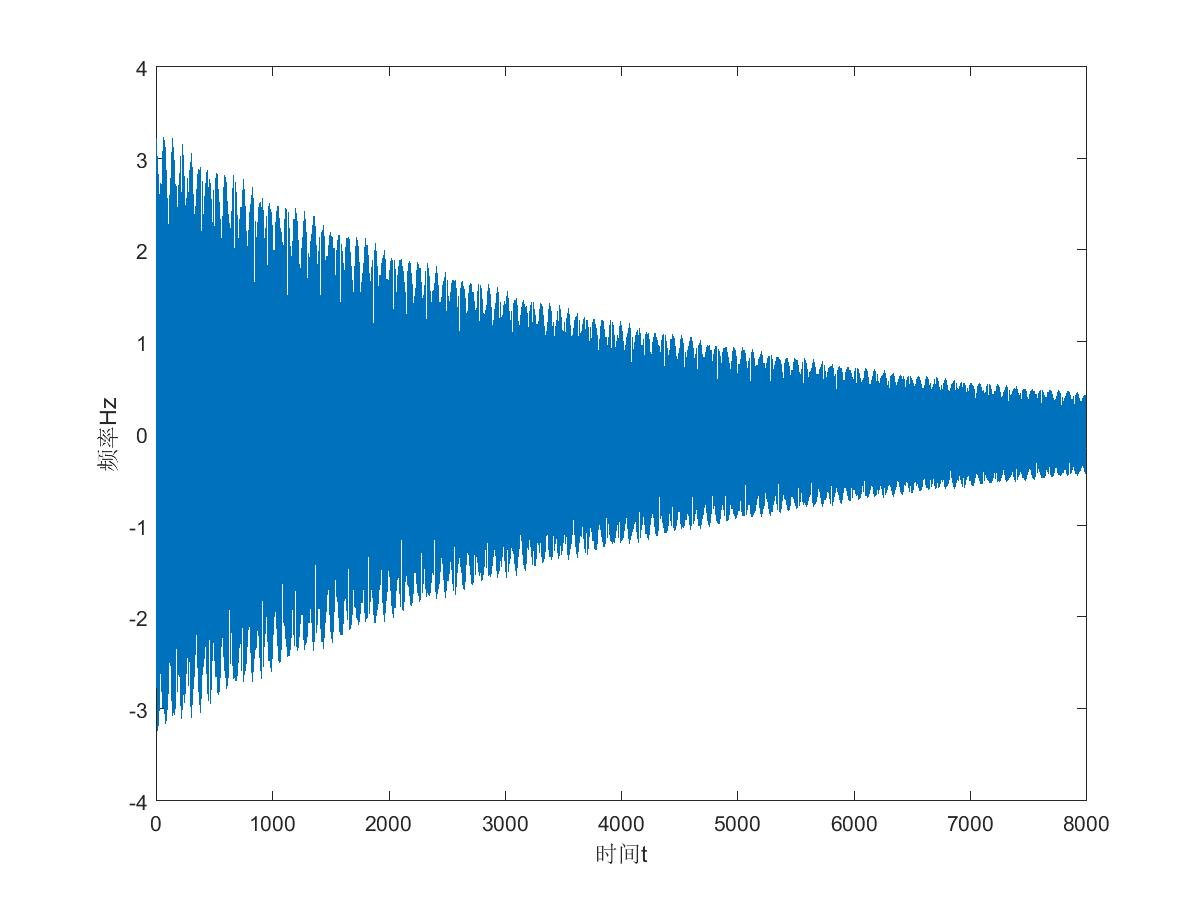
\includegraphics[width=6cm]{../source/generate_jpg/tone_g.jpg}\caption{生成的G时域域图}\label{gt}
\end{figurehere}
这些信号在聆听时相对来讲还是比较接近真实情况的曲调的。
\subsubsection{简单的音乐}
\indent本文主要尝试利用Matlab生成了欢乐颂和清华校歌这两首曲子。这两首曲子特点是没有例如连音之类的较为复杂的音乐技巧。
同时声音的曲调变化范围也相对较为狭窄,所以便于使用Matlab进行生成。
这两首曲子的时域信号与频域时域综合信号如下所示:
\begin{figurehere}
\centering
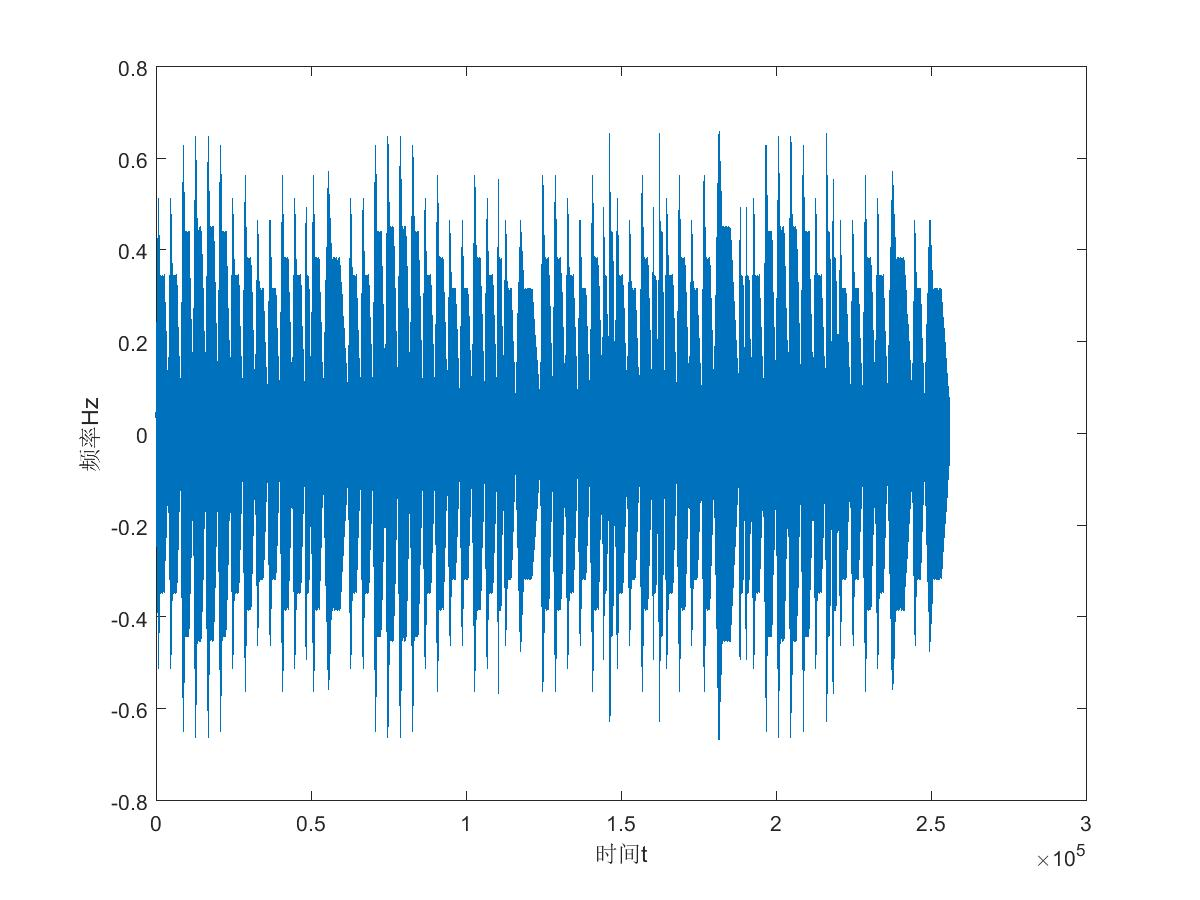
\includegraphics[width=6cm]{../source/generate_jpg/song_of_happiness1.jpg}\caption{欢乐颂时域}\label{happinesst}
\end{figurehere}
\begin{figurehere}
\centering
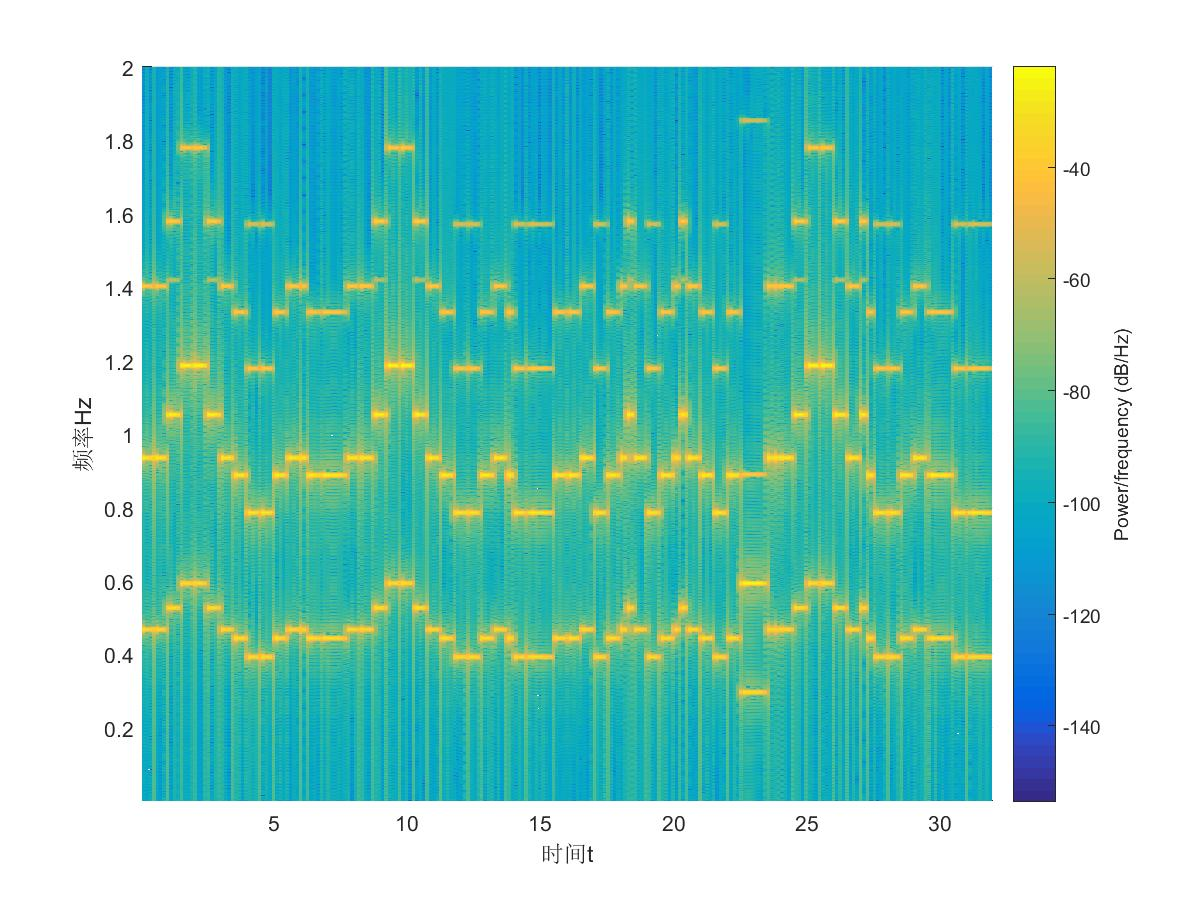
\includegraphics[width=6cm]{../source/generate_jpg/song_of_happiness2.jpg}\caption{欢乐颂时域频域综合图} \label{happiness}
\end{figurehere}
\begin{figurehere}
\centering
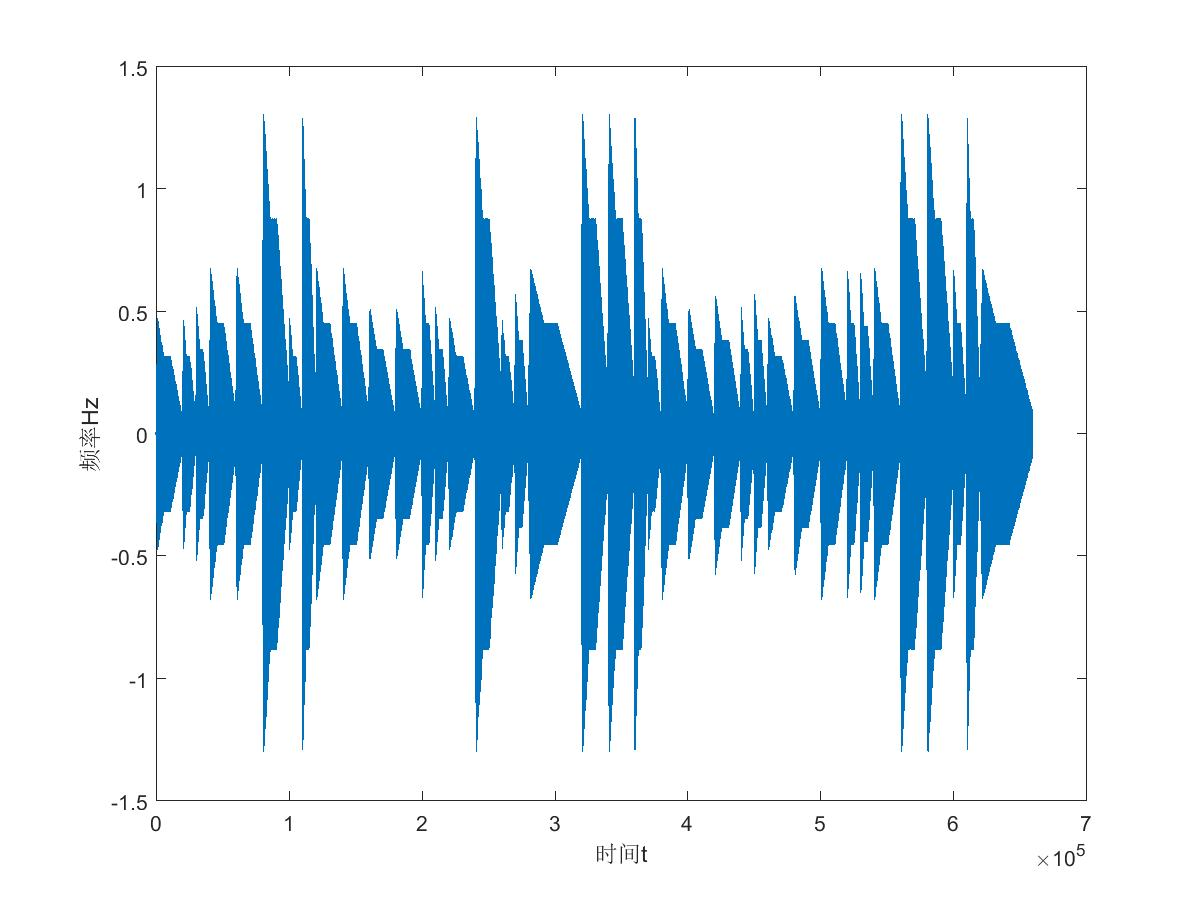
\includegraphics[width=6cm]{../source/generate_jpg/song_of_thu1.jpg}\caption{清华校歌时域图}\label{thut}
\end{figurehere}
\begin{figurehere}
\centering
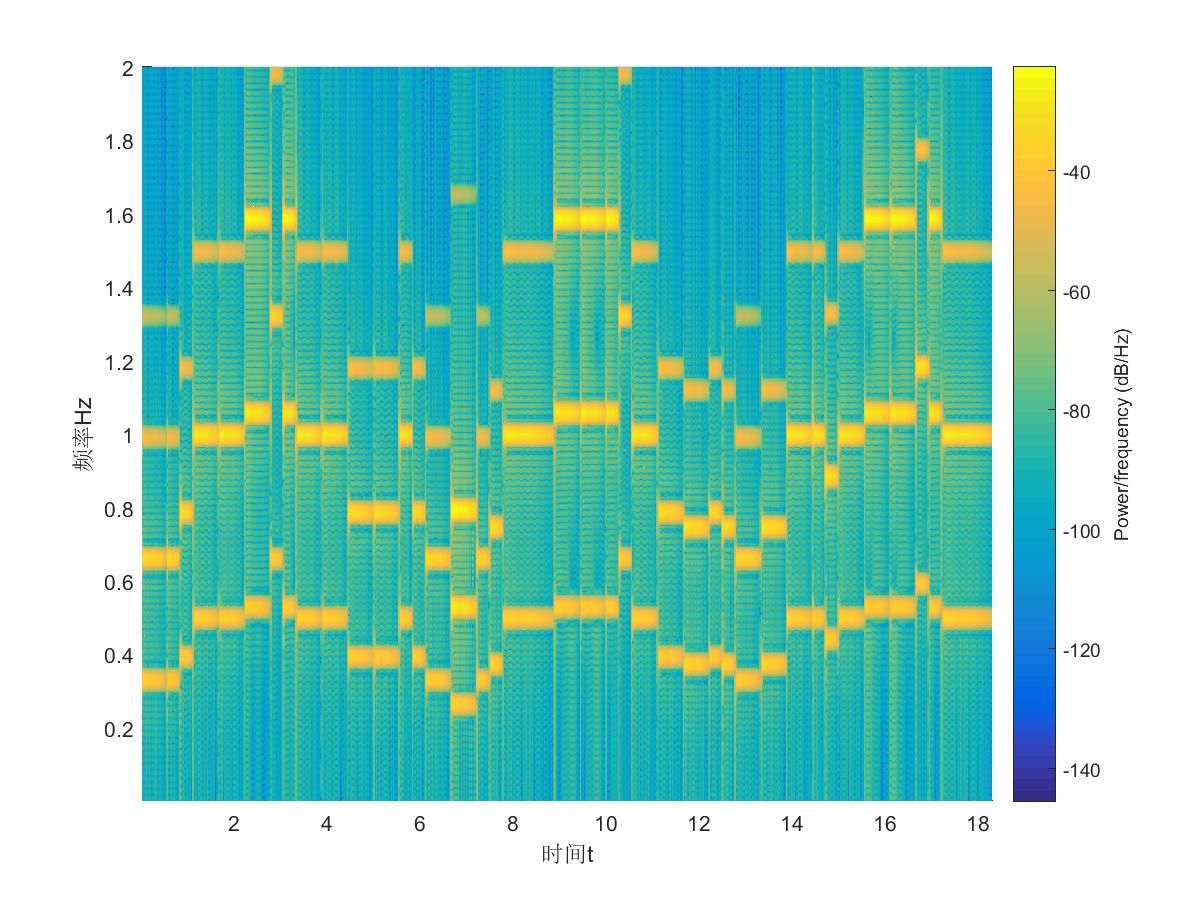
\includegraphics[width=6cm]{../source/generate_jpg/song_of_thu2.jpg}\caption{清华校歌频域时域域综合图}\label{thu}
\end{figurehere}
而产生的音乐听起来可以大致感受的到音调,音色也大致接近,但是在两个音符过度部分仍有一些不自然。\\


\section{结论}
\indent 本文主要讨论如何利用Matlab生成钢琴曲。采用的方法是先利用Matlab分析标准的钢琴音信号,记录下频率特征,从而能够
反向生成出对应的钢琴音调。在通过还原简谱的方式,并加上我们改进的包络线降噪方式实现了较好的还原钢琴曲信号的结果。未来能够
改进的就是寻找更好的方式降低不同音符之间过度之时的不自然之处,使之更加接近真实的钢琴曲。
\end{multicols}
\section{参考文献}
[1]:http://blog.sina.com.cn/s/blog_7e1870780100ynw1.html

[2]:http://blog.sina.com.cn/s/blog_891a4b2c0101f81i.html
\section{源码和声音文件仓库}
https://github.com/wutb15/piano
\clearpage
\end{CJK*}
\end{document}